\section{Experimental Evaluation}
\label{sec:results}

\vspace{-1mm}
We have gathered preliminary performance results using a prototype
implementation of \pdht running on the Portals reference
implementation~\cite{portals-code}.  Results were gathered on the Comet
system at the San Diego Supercomputer Center with access provided
through the Extreme Science and Engineering Discovery Environment (XSEDE)
program.  Comet contains nodes with several configurations; for our
experiments, we used the Intel\regtm Xeon\regtm E5 nodes.  There are 1944 such
nodes, which are constructed from Dell\othertm PowerEdge\othertm C6320 servers
containing dual 12-core Intel\regtm Xeon\regtm E5-2680 processors and 128
gigabytes of memory.  Nodes are connected using a Mellanox\othertm FDR 56 Gb/s
InfiniBand\othertm fabric.


%Our first experiment, shown in Figure~\ref{fig:throughput}, measures
%the overall throughput of a set of distinct remote read operations on
%the distributed key/value store. This figure shows that \pdht scales
%reasonably, with communication volume increasing as processor counts
%grow. 

%An initial study of the performance of \pdht can be seen in
%Figure~\ref{fig:throughput}. This figure shows that \pdht reads scale
%reasonably, with communication volume increasing as processor counts
%grow. This experiment was run on one core per node, with the hash
%function configured to ensure all reads occur remotely, over the
%Infiniband\othertm interface.

As shown in Figure~\ref{fig:throughput}, we measure the weak scaling
of \pdht read operations on the key/value store by examining the
overall throughput of the system. Each process owns a fixed number of
hash table elements which are read by a neighboring process. The
system performs as expected under weak scaling, with overall system
throughput increasing with the number of processes involved. Of
particular interest, is the observation that throughput decreases as
the number of local hash table elements increases. Lower throughputs
with a larger number of elements imply higher overheads
within the message matching process in the Portals runtime.

To verify this, we measure the performance of retrieving elements from
the \pdht with respect to the number of elements on each process.
These results are shown in Figure~\ref{fig:mlen} and provide an
initial characterization of the lookup cost associated with our \pdht
implementation.  In contrast with traditional PGAS approaches,
building a remotely accessible key/value store on top of a mechanism
intended to support MPI message matching can add new overheads.  In
particular, the Portals message processing engine must traverse the
active match list until an ME that matches the given query is located.
In cases where the element does not exist, the Portals layer must
reach the end of the list to make this conclusion.  Thus, there is a
list traversal overhead that is proportional to the number of elements
visited before finding a match.

\begin{figure}
    \centering
    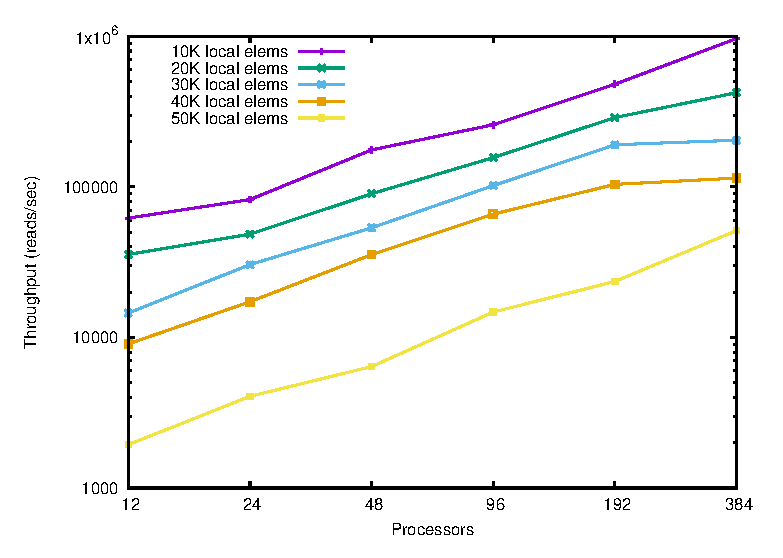
\includegraphics[width=.9\linewidth]{plots/throughput}
    %\caption{System throughput for a range of local volume (entries per node).}
    \caption{Aggregate system throughput for active list lengths of 10,000 to 50,000 local elements (8 byte elements)}
    \label{fig:throughput}
\end{figure}

\begin{figure}
    \centering
    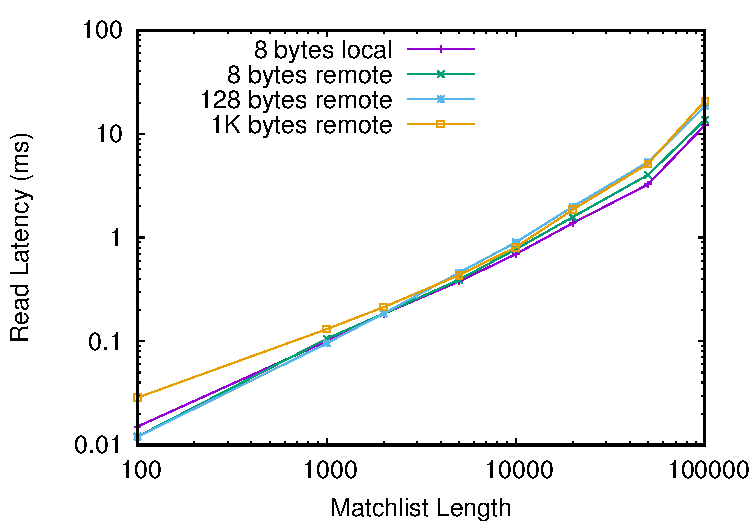
\includegraphics[width=.95\linewidth]{plots/mlen}
    %\caption{Read operation latency versus list depth for various size entries.}
    \caption{Latency for various size read operations measured over a range of active list (Portals matchlist) lengths. For this experiment, the expected matching depth of a list of length $L$ is $L/2$.}
    \label{fig:mlen}
\end{figure}

The Portals layer must maintain each matching list as an ordered list in order
to preserve MPI message ordering semantics.  However, we observe that this
ordering is not required by \pdht.  Also, in contrast to MPI applications,
where typical communication patterns result in short matching lists or in
matching occurring near the head of the list, \pdht necessarily generates long
matching lists with an expected matching depth of the midpoint in the list.
Thus, we identify this overhead as a key challenge to supporting such models
and plan to investigate solutions in our future work.
%%% Local Variables:
%%% mode: latex
%%% TeX-master: "paper"
%%% End:
